\begin{frame}[t]{What is a Biometric?}
	\topline
    \begin{itemize}
    	\item \textcolor{navy_theme}{\textbf{Examples of Biometric Traits}}
			\begin{figure}[!ht]
				\centering 
				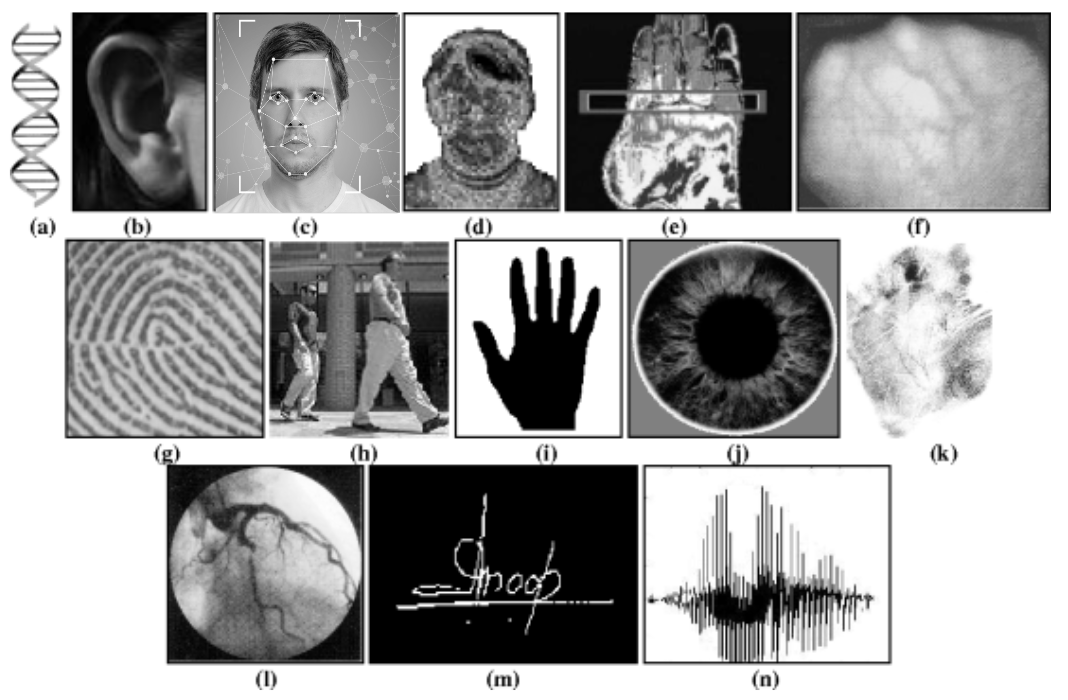
\includegraphics[width=0.70\textwidth]{images/Examples of biometric characteristics.png}
				\caption{(a) DNA profiling, (b) ear shape, (c) facial features, (d) facial thermograph, (e) hand thermograph, (f) hand vein profile, (g) fingerprints, (h) gait, (i) hand geometry, (j) iris, (k) palmprint, (l) retina scans, (m) signature, and (n) voice.}
				\label{fig:bio_ex}
			\end{figure}
		\end{itemize}
\end{frame}

\begin{frame}[t]{How to decide on a Biometric?}
	\topline
	\centering
    \begin{itemize}
		\item Feasibility of a biometric traits \cite{Unar2014}
		\vspace{1em}
		\begin{itemize}
			\setlength\itemsep{1em}

		    \item \textit{Universality}
			% : present in every person
			% \vspace{0.25cm}
		    \item \textit{Distinctiveness}
			% : two people having the given trait should have sufficient difference
			% \vspace{0.25cm}
		    \item \textit{Collectability}
			% : the trait should be fairly easy to collect and quantify/feature extraction
			% \vspace{0.25cm}
		    \item \textit{Permanence}
			% : over time, the trait should not change (eg. as a person ages)
			% \vspace{0.25cm}
		    \item \textit{Performance}
			% : availability of resources constraints in data collection, and the guarantee of high accuracy when matching
			% \vspace{0.25cm}
		    \item \textit{Acceptability}
			% : the willingness of people to submit the trait and privacy risks involved 
			% \vspace{0.25cm}
		    \item \textit{Circumvention}
			% : prone to imitation or fraudulent attempts to mimic the trait 
		\end{itemize}
	\end{itemize}
\end{frame}

\begin{frame}[t]{Comparison of Biometric Traits}
	\topline
	\begin{itemize}
		\item Feasibility comparison of biometric traits \cite{Jain2004}
			\begin{figure}[!ht]
				\centering 
				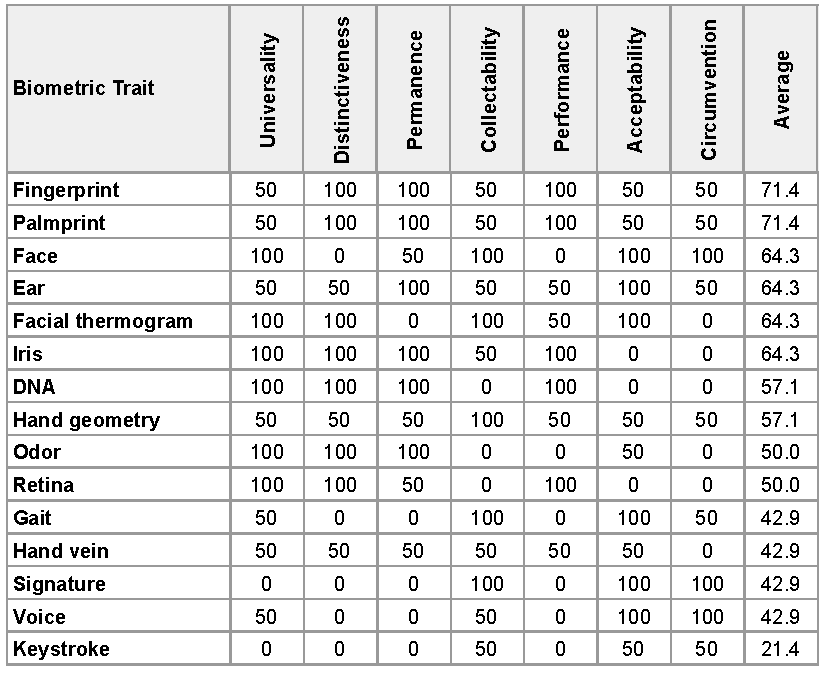
\includegraphics[width=0.60\textwidth]{images/Comparison of Various Biometric Technologies Based on the Perception_numbers.pdf}
				\caption{High=100, Medium=50, Low=0\cite{Jain2004} }
				% \caption{Block Diagram of a generic biometric system along with its subsystems \cite{Leniski2003}}
				% \label{fig:bio_sys_block}
			\end{figure}
	\end{itemize}
\end{frame}


\begin{frame}[t]{Diffrent Modalities of Biometric}
	\topline
    \begin{itemize}
    	\item \textcolor{navy_theme}{\textbf{Biometric Modalities}}
			\begin{figure}[!ht]
				\centering 
				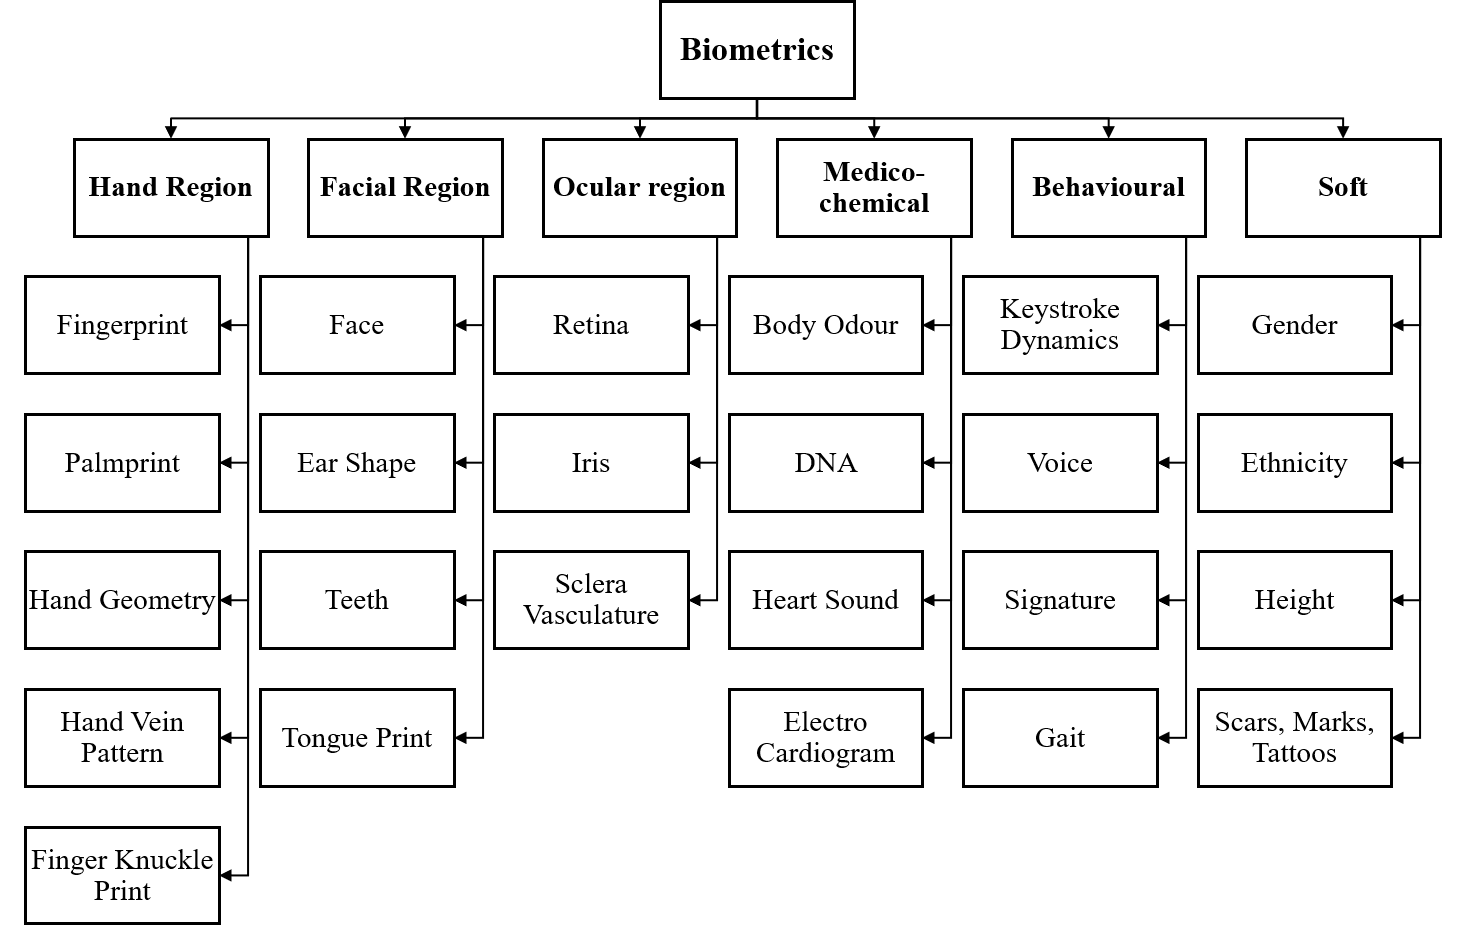
\includegraphics[width=0.90\textwidth]{images/Classification of biometric modalities.png}
				\caption{Classification of Biometric Modalities}
				\label{fig:bio_class_mod}
			\end{figure}
	\end{itemize}
\end{frame}

\begin{frame}[t]{Biometric Authentication System}
	\topline
    \begin{itemize}
		% \setlength\parsep{2em}
		% \begin{itemize}[parsep=2em]
		\setbeamercovered{transparent}
    	\item \textcolor{navy_theme}{\textbf{Working modes of biometric authentication system}}
		\vspace{1em}
			\begin{itemize}
				\setlength\itemsep{1.5em}
				% \vspace{0.35cm}
				\item<1> Identification System
				% \vspace{0.35cm}
				\item<2> Recognition System
			\end{itemize}
	\end{itemize}
\end{frame}

\begin{frame}[t]{Biometric Authentication System}
	\topline
    \begin{itemize}
    	\item \textcolor{navy_theme}{\textbf{Biometric Authentication System}}
			\begin{figure}[!ht]
				\centering 
				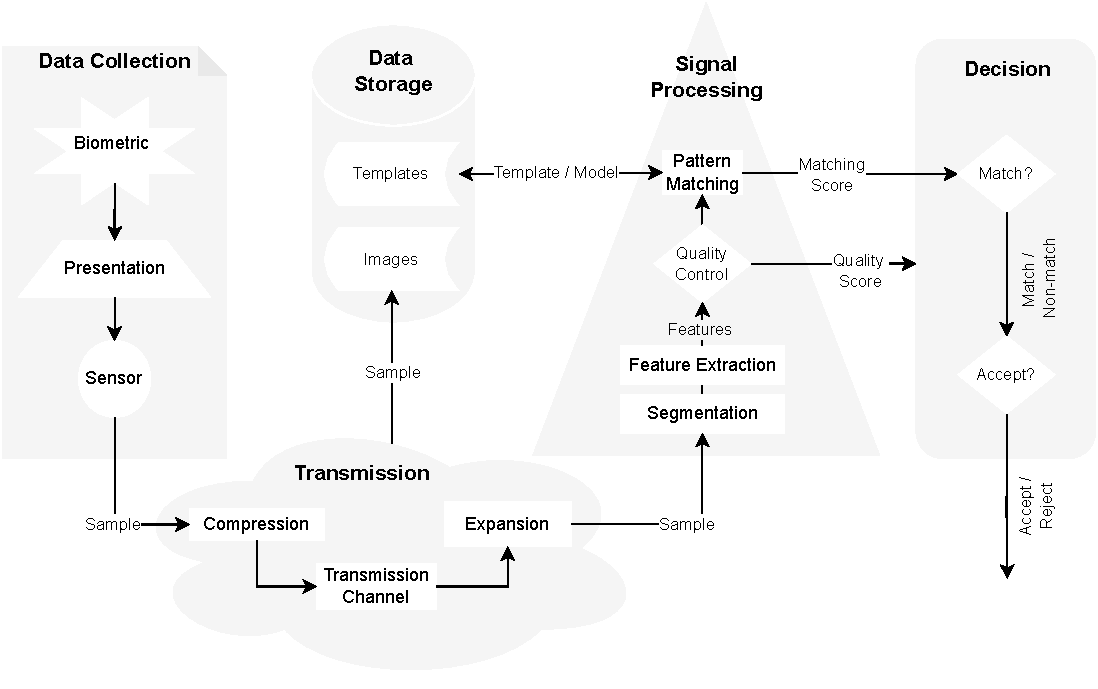
\includegraphics[width=0.85\textwidth]{images/Block diagram of a generic biometric system.pdf}
				\caption{Block Diagram of a Biometric Authentication System}
				\label{fig:bio_sys}
			\end{figure}
	\end{itemize}
\end{frame}


\begin{frame}[t]{Database Idexing}
	\topline
    \begin{itemize}
    	\item \textcolor{navy_theme}{\textbf{Indexing Techniques}}
			\begin{figure}[!ht]
				\centering 
				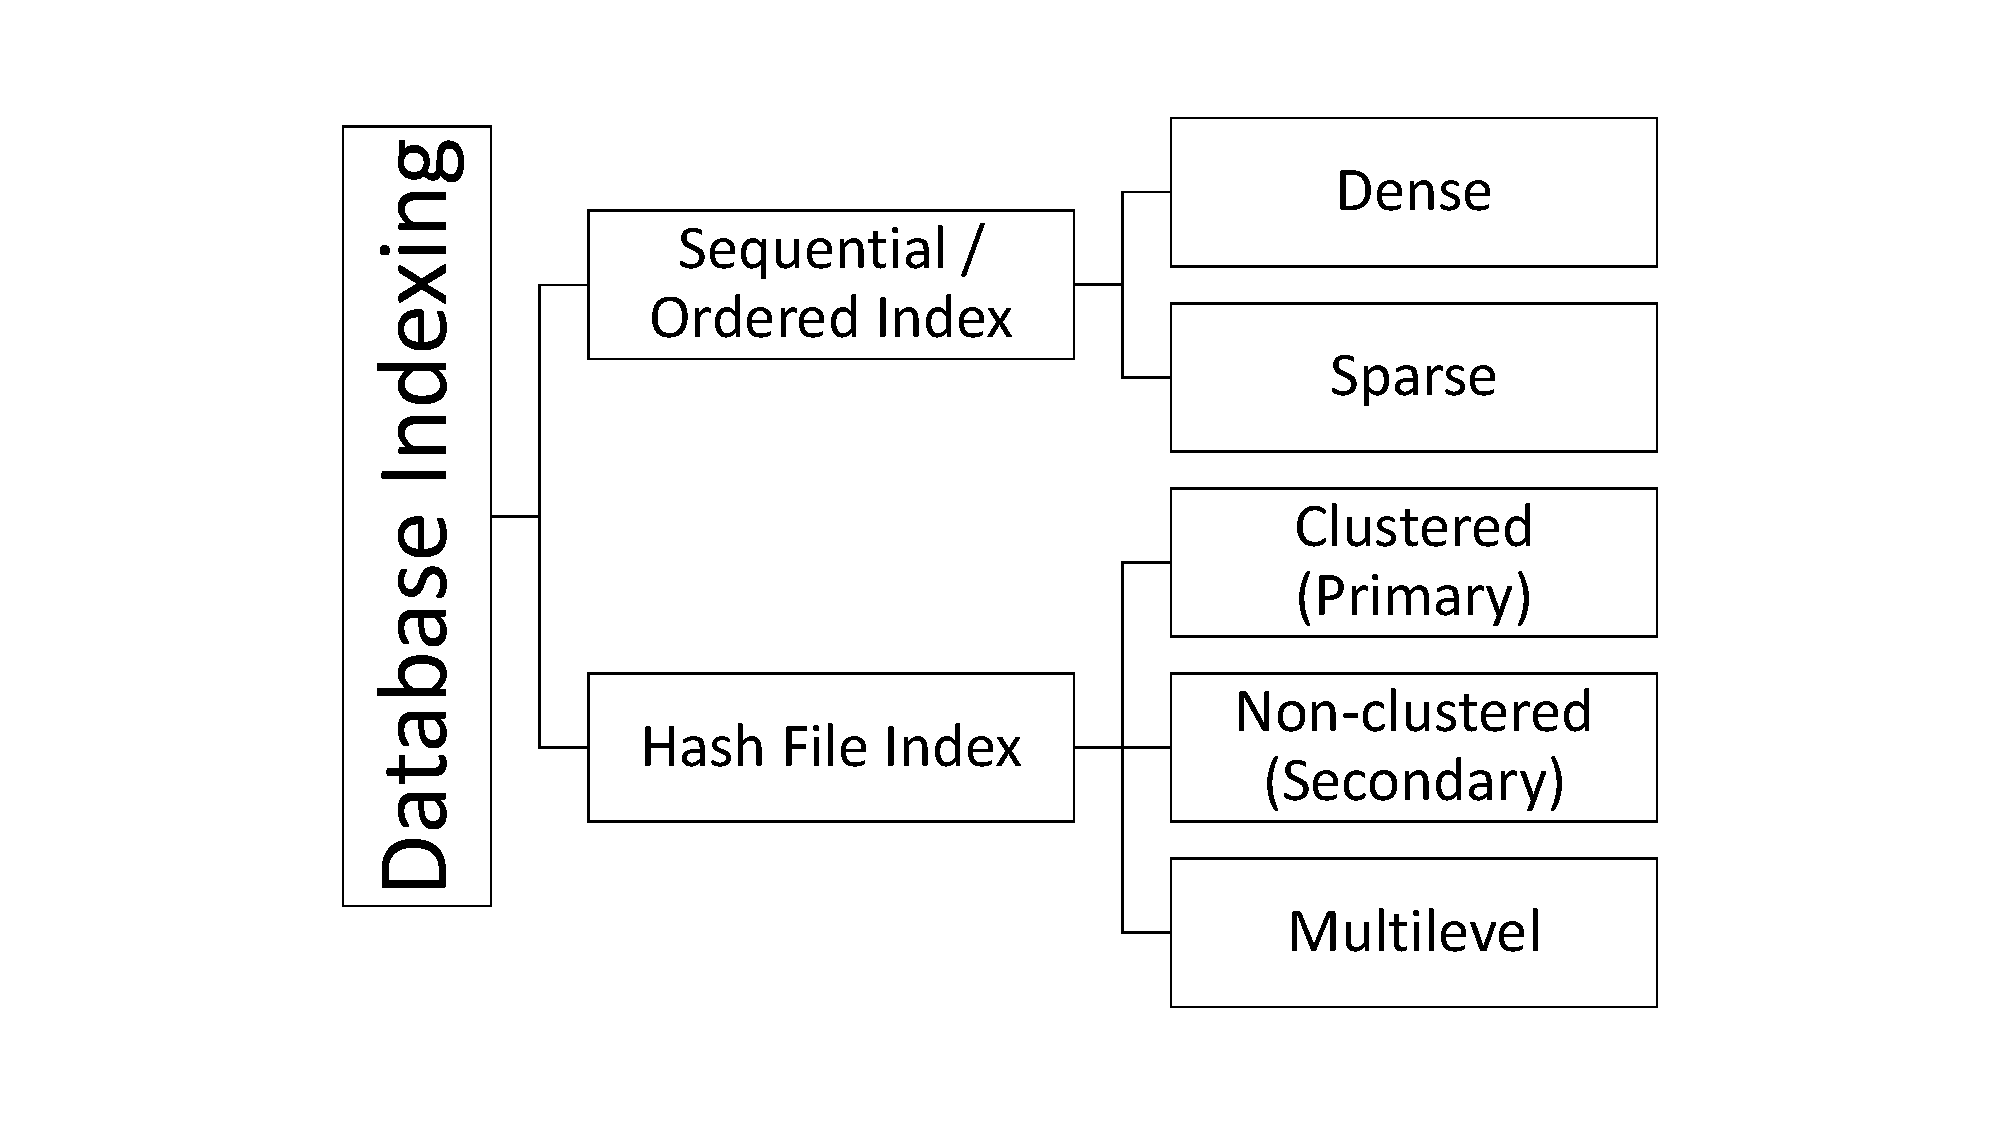
\includegraphics[width=0.90\textwidth]{images/Classification of database indexing.pdf}
				\caption{Classification of Database Indexing}
				\label{fig:indexing}
			\end{figure}
	\end{itemize}
\end{frame}

\begin{frame}[t]{Indexing Techniques}
	\topline
    \begin{itemize}
		\item \textcolor{navy_theme}{\textbf{Common Indexing Techniques}}
		\vspace{1em}
			\begin{itemize}
				\setlength\itemsep{1.5em}
				
				% \vspace{0.25cm}

				\item Dense Index
				% \vspace{0.25cm}
				\item Sparse Index
				% \vspace{0.25cm}
				\item Secondary Index
				% \vspace{0.25cm}
				\item Hashing
				% \vspace{0.25cm}
				\item B-Tree (B+ Tree)
				% \vspace{0.25cm}
				\item kd-Tree
			\end{itemize}
	\end{itemize}
\end{frame}

\begin{frame}[t]{Indexing of Biometric Data}
	\topline
    \begin{itemize}
    	\item \textcolor{navy_theme}{\textbf{Indexing of Biometric Data}}
    	\vspace{0.5em}
			\begin{figure}[!ht]
				\centering 
				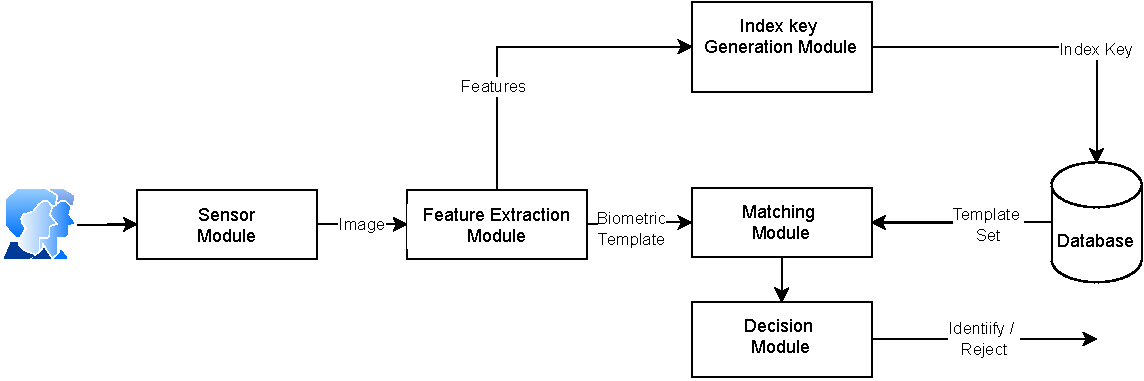
\includegraphics[width=0.90\textwidth]{images/steps_in_identification_with_indexing.drawio.pdf}
				\caption{Steps in Biometric Identification with indexing}
				\label{fig:bio_indexing}
			\end{figure}
	\end{itemize}
\end{frame}

